\subsection{Class Diagram}

%\includegraphics[]{ClassDiagram.pdf}

%Describe here the class diagram of your project

\subsubsection{Login}
\begin{figure}[H]
    \centering
    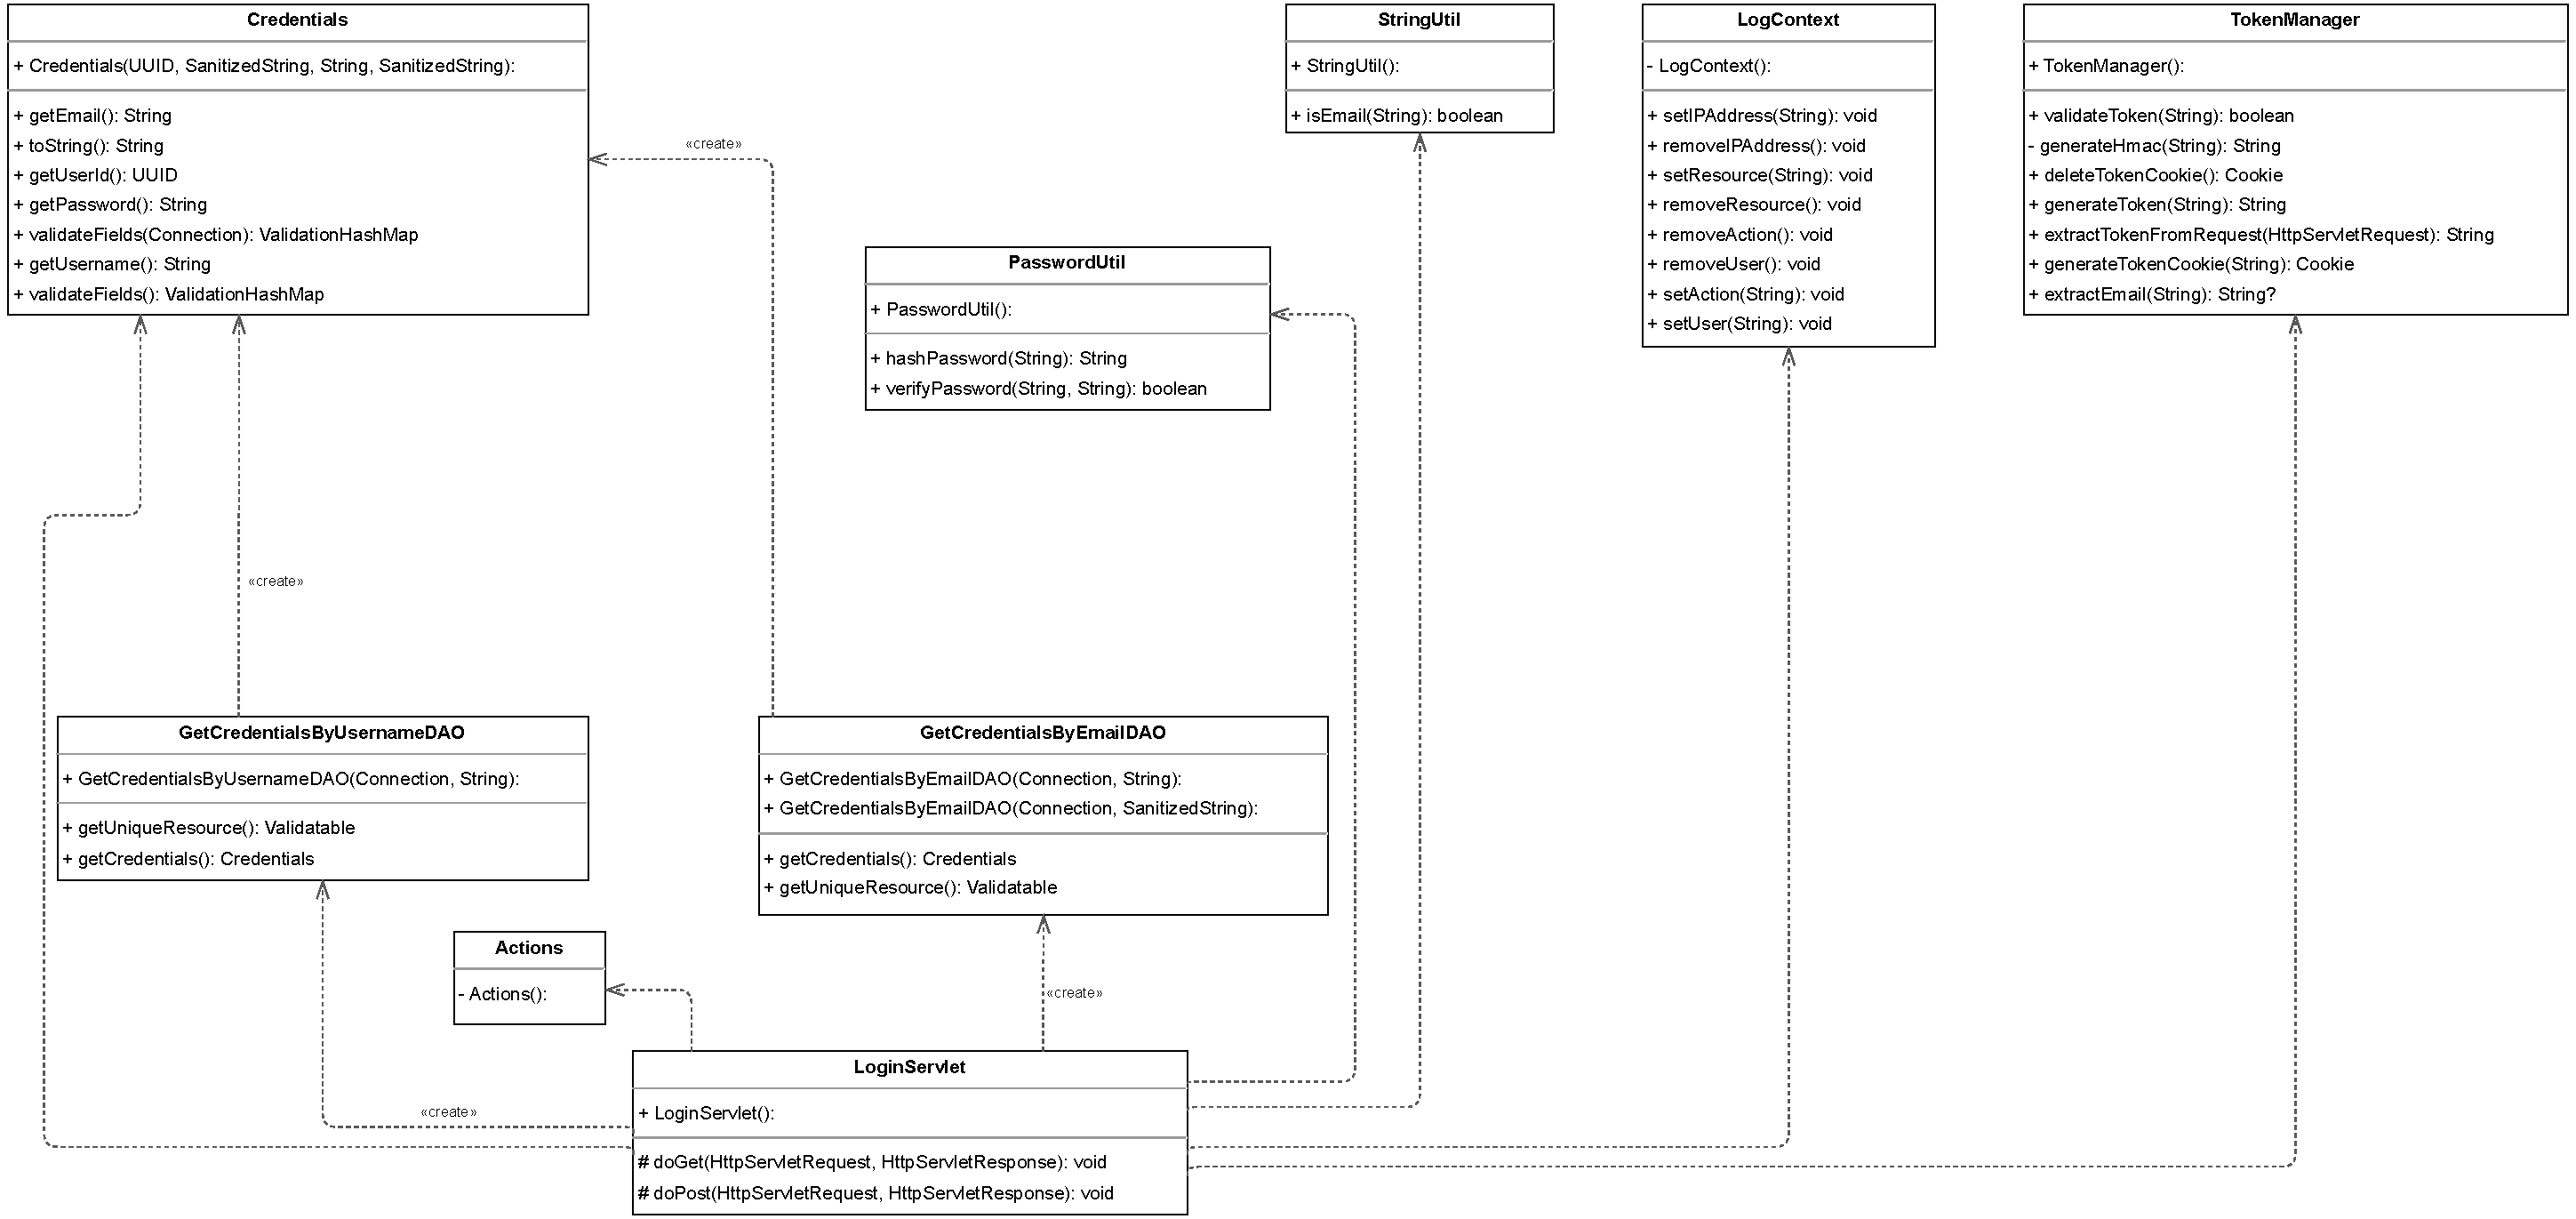
\includegraphics[width=0.9\textwidth]{images/class_diagrams/Login_classdiagram.pdf}
    \caption{Login Class Diagram}
\end{figure}

The class diagram captures the core components involved in the login functionality of the application: the domain model for user credentials, the data‐access layer to retrieve those credentials, the servlet that orchestrates the login flow, and several utility classes supporting validation, password handling, token management and logging.

At the center is LoginServlet, a subclass of HttpServlet that overrides the doGet and doPost methods. Upon receiving a request, it first uses StringUtil to determine whether the supplied identifier is an email address or a username. Based on this, it instantiates either GetCredentialsByEmailDAO or GetCredentialsByUsernameDAO, passing along a JDBC Connection and the raw or sanitized identifier. Once the Credentials object is retrieved, LoginServlet invokes PasswordUtil to verify the submitted password. If authentication succeeds, it delegates to TokenManager to generate an authentication token (and corresponding cookie), and uses LogContext to record the action, associating the user, resource (“login”), and client IP for auditing. Finally, it forwards or redirects the user according to the outcome of these operations.

The two DAO classes, GetCredentialsByEmailDAO and GetCredentialsByUsernameDAO, encapsulate all data-base interactions needed to fetch a single Credentials instance. Each DAO constructor accepts a Connection and either a plain String or a SanitizedString, and both implement a getUniqueResource() method (returning a Validatable) alongside getCredentials(), which returns the populated Credentials domain object. This separation ensures that the servlet remains agnostic of the underlying query logic and focuses solely on control flow and error handling.
The Credentials class itself models the essential fields for authentication: a UUID user ID, a username and password (as raw String), and an email (wrapped in SanitizedString). It provides accessor methods (getEmail(), getUsername(), getUserId(), getPassword()), a toString() override, and two validateFields() methods—one that performs in-memory checks, and another that can apply database‐backed validations via a Connection, returning a ValidationHashMap of any detected issues.

Supporting this flow are four smaller utility classes:
\begin{itemize}
    \item PasswordUtil, responsible for hashing plaintext passwords (hashPassword(String)) and verifying a candidate password against a stored hash (verifyPassword(String, String)).
    \item StringUtil, offering a single method isEmail(String) to distinguish email addresses from usernames.
    \item TokenManager, which encapsulates all HMAC‐based token operations (generation via generateHmac(String), token creation and validation, extraction from HTTP requests, and cookie creation/deletion).
    \item LogContext, which maintains a thread‐local logging context, with setters and removers for IP address, resource name, action, and user, ensuring that every step of the login process can be traced in the application logs.
\end{itemize}

%%%%%%%%%%%%%%%%%%%%%%%%%%%%%%%%%%%%%%%%%%%%%%%
\subsubsection{Settings}
\begin{figure}[H]
    \centering
    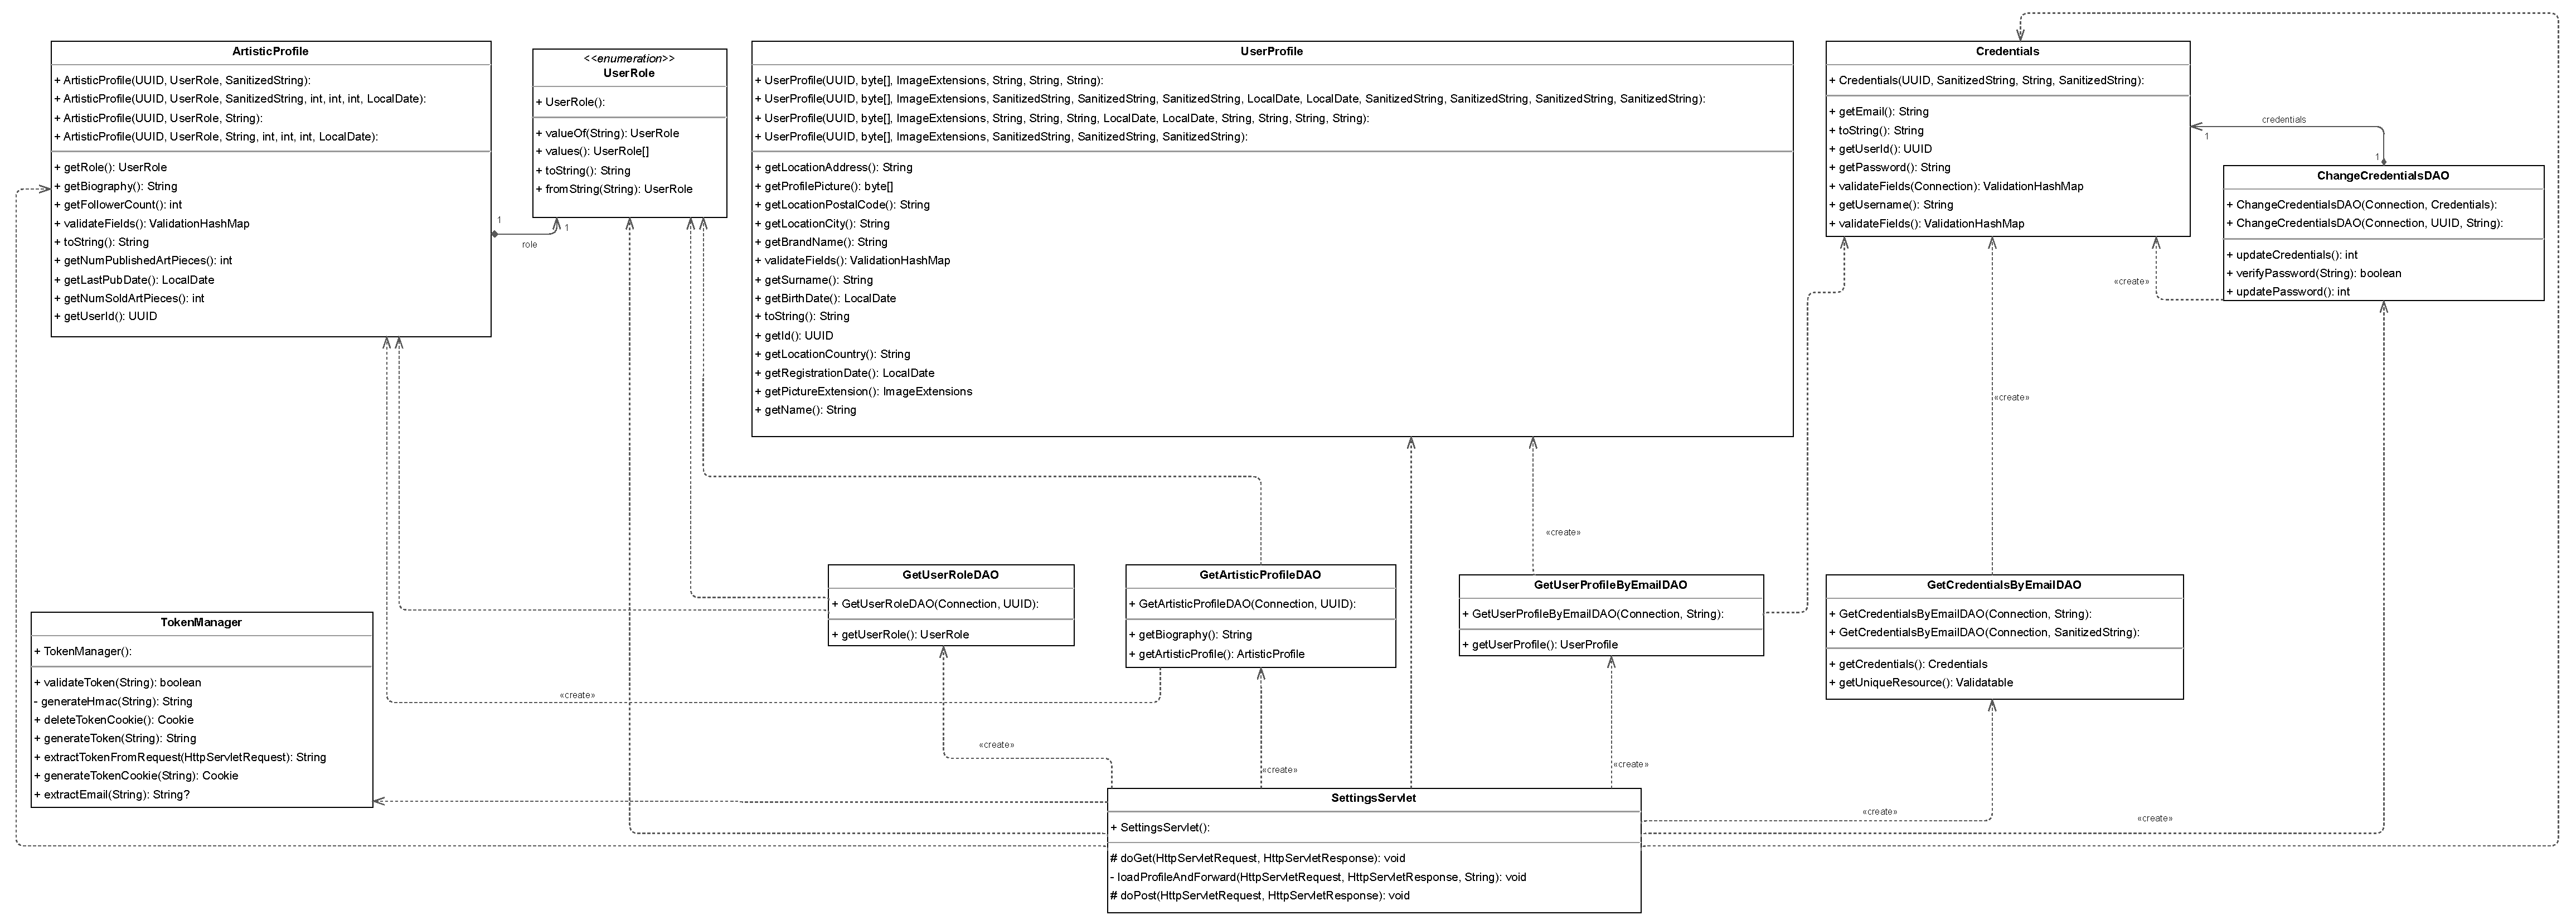
\includegraphics[width=0.9\textwidth]{images/class_diagrams/Settings_classdiagram.pdf}
    \caption{Settings Class Diagram}
\end{figure}

The class diagram models all the pieces involved in the “Settings” feature of the application: changing credentials, viewing/editing a user’s profile (including special “artistic” profiles), and enforcing role‐based access. It centers on a single servlet—SettingsServlet—subclassing HttpServlet, which implements both doGet and doPost (and a private helper loadProfileAndForward) to handle all settings‐related requests.

SettingsServlet:
\begin{itemize}
    \item doGet: Uses TokenManager to extract and validate the auth token from the incoming request, then pulls out the user’s email.
    Instantiates GetCredentialsByEmailDAO and GetUserRoleDAO (each taking a JDBC Connection plus the email or user UUID) to fetch the user’s Credentials and UserRole.
    Calls GetUserProfileByEmailDAO to load the basic UserProfile.
    If the UserRole equals ARTIST, also invokes GetArtisticProfileDAO to retrieve the user’s ArtisticProfile (biography, follower counts, publication stats, etc.).
    Delegates to loadProfileAndForward(), passing all retrieved model objects to the view layer.
    \item doPost: Handles updates submitted by the user. For credential changes, it creates a ChangeCredentialsDAO (with either a Credentials object or user‐ID plus new password), then calls verifyPassword(old) followed by updatePassword() or updateCredentials(). Any validation errors bubble back as a ValidationHashMap. (Other profile‐update DAOs aren’t shown in this diagram.)
\end{itemize}

Data‐Access Objects (DAOs):
\begin{itemize}
    \item GetCredentialsByEmailDAO / GetUserRoleDAO / GetUserProfileByEmailDAO / GetArtisticProfileDAO each wrap the SQL needed to fetch one resource by key. They expose a getXxx() method (e.g. getCredentials(), getUserRole(), getUserProfile(), getArtisticProfile()) and, where applicable, a getUniqueResource(): Validatable for shared validation logic.
    \item ChangeCredentialsDAO additionally provides verifyPassword(String) and updatePassword() along with a generic updateCredentials().
\end{itemize}

Domain Model Classes:
\begin{itemize}
    \item Credentials: holds UUID userId, username, email (SanitizedString), and password; offers getters, toString(), and two validateFields() overloads (in‑memory and DB‐backed).
    \item UserProfile: aggregates personal data—UUID id, profile picture byte[] + ImageExtensions, name/surname, birthDate, registrationDate, address fields, etc.—with getters and a validateFields() method.
    \item ArtisticProfile: for users with the ARTIST role, extends the generic profile with biography, followerCount, numPublishedArtPieces, numSoldArtPieces and lastPubDate; also implements validateFields().
\end{itemize}

Utilities and Enumeration:
\begin{itemize}
    \item TokenManager: encapsulates all HMAC‐based token logic—generateHmac(), generateToken(), validateToken(), plus cookie creation/deletion and token extraction from requests.
    \item UserRole (enum): defines all possible roles (e.g. ARTIST, USER, ADMIN), with standard values(), valueOf(), and a custom fromString() for safe parsing.
\end{itemize}

%%%%%%%%%%%%%%%%%%%%%%%%%%%%%%%%%%%%%%%%%%%%%%%
\subsubsection{Upload Art Piece}
\begin{figure}[H]
    \centering
    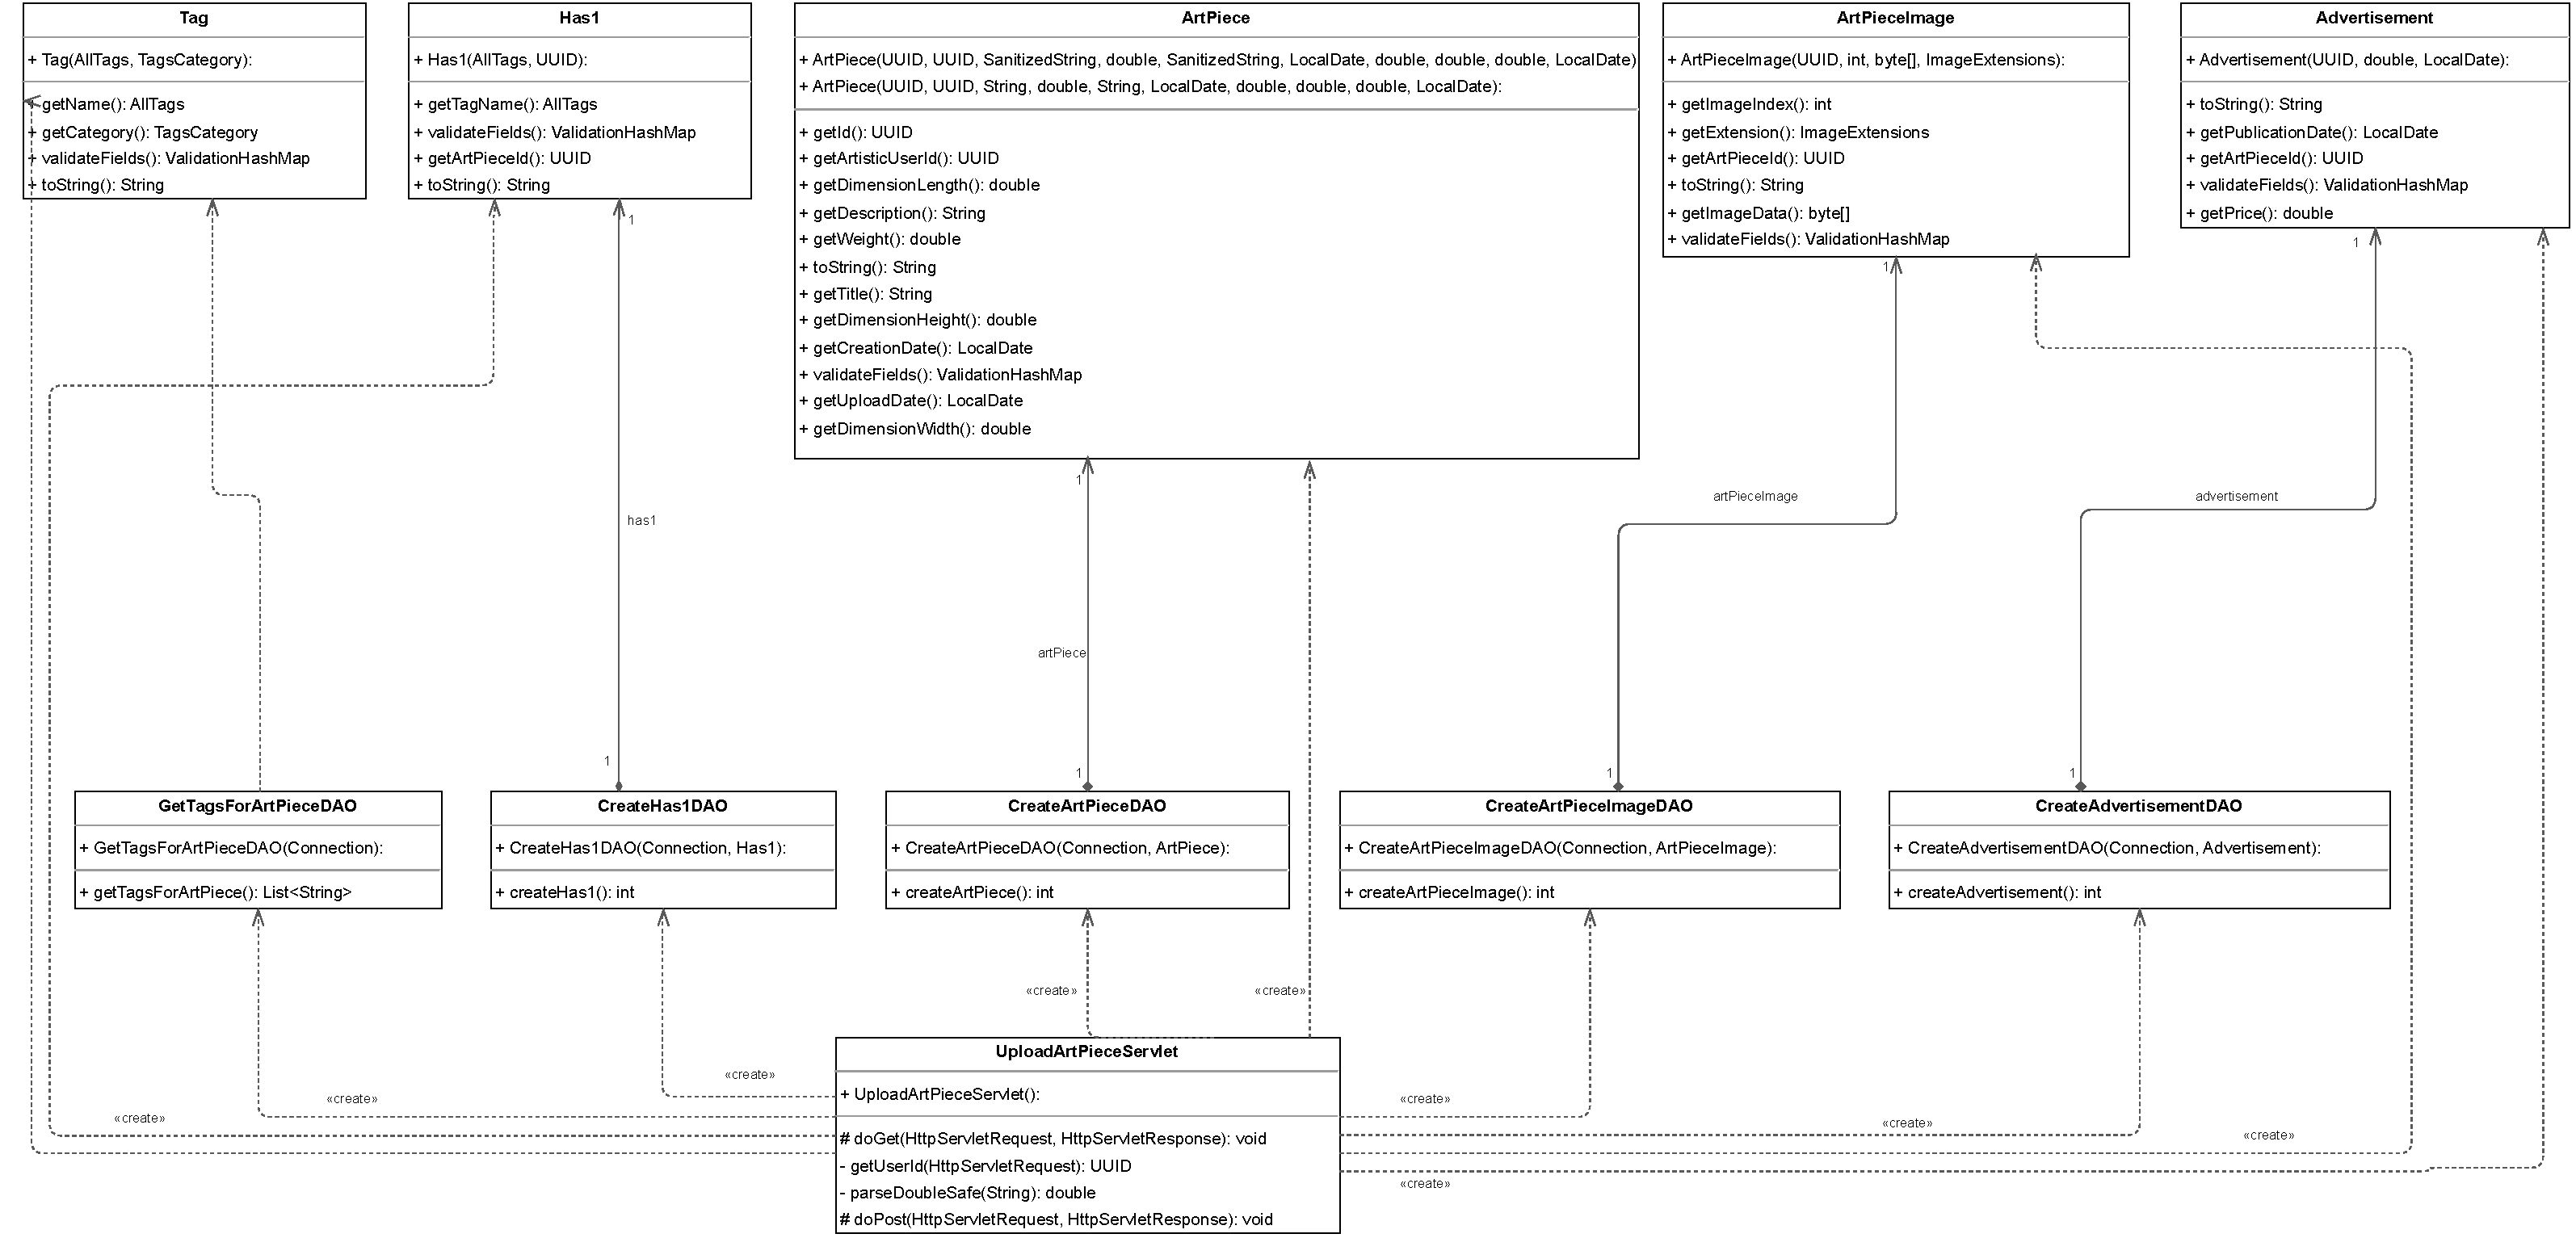
\includegraphics[width=0.9\textwidth]{images/class_diagrams/UploadArtPiece_classdiagram.pdf}
    \caption{Upload Art Piece Class Diagram}
\end{figure}


The class diagram models all the pieces involved in uploading a new art piece—its metadata, images, tags and an optional advertisement—centered on a single servlet and a set of DAOs that persist each piece of data. At its heart is UploadArtPieceServlet, a subclass of HttpServlet that implements both doGet(HttpServletRequest, HttpServletResponse) and doPost(HttpServletRequest, HttpServletResponse), plus two private helpers:
\begin{itemize}
    \item getUserId(HttpServletRequest): extracts the authenticated user’s UUID from the session or token.
    \item parseDoubleSafe(String): safely converts form‐input strings into doubles, handling invalid or empty values gracefully.
\end{itemize}

In doGet, the servlet creates a GetTagsForArtPieceDAO (passing in a Connection), invokes getTagsForArtPiece() to fetch all allowed tag names, and forwards these to the JSP for rendering the upload form. In doPost, it reads all form parameters—title, description, creation date, price, weight, dimensions, selected tags, uploaded image files, and advertisement details—and then orchestrates persistence by instantiating and invoking the appropriate DAO for each step. Once all DAOs succeed, it redirects (or forwards) the user based on the outcome.

Persistence is fully delegated to five dedicated DAO classes, each following a one‐class/one‐operation pattern. All DAO constructors accept a JDBC Connection and the domain object (or association) to be created, exposing a single method that executes the SQL and returns an update count:
\begin{itemize}
    \item CreateArtPieceDAO → createArtPiece(): int
    \item CreateArtPieceImageDAO → createArtPieceImage(): int
    \item CreateAdvertisementDAO → createAdvertisement(): int
    \item CreateHas1DAO → createHas1(): int
    \item GetTagsForArtPieceDAO → getTagsForArtPiece(): List<String>
\end{itemize}
This clear separation keeps SQL details out of the servlet and ensures each DAO is responsible for exactly one table or relationship.

The domain model is composed of four main classes, each with constructors, getters, a toString(), and a validateFields(): ValidationHashMap method for business‐rule enforcement:
\begin{itemize}
    \item ArtPiece: encapsulates an art work’s core metadata—UUID id, UUID artisticUserId, title (SanitizedString), price (double), description (SanitizedString), creationDate (LocalDate), weight (double), dimensionHeight/dimensionWidth/dimensionLength (double), and uploadDate (LocalDate).
    \item ArtPieceImage: represents each image file for an art piece, storing UUID artPieceId, an imageIndex (int), the raw byte[] imageData, and its ImageExtensions.
    \item Advertisement: links a piece to a marketplace listing via UUID artPieceId, a price (double), and publicationDate (LocalDate).
    \item Has1: models the association between an art piece and a tag, with fields tagName (AllTags enum) and UUID artPieceId.
\end{itemize}

Tagging is supported by two additional types:
\begin{itemize}
    \item Tag, constructed from an AllTags constant and a TagsCategory enum, encapsulates the name/category of each tag and provides validation.
    \item The AllTags and TagsCategory enumerations list every permissible tag name and its grouping, ensuring compile‐time safety and consistent use throughout the upload workflow.
\end{itemize}
